\documentclass{article} 
\usepackage[utf8]{inputenc}
\usepackage{ amssymb, systeme,   float, graphicx, fontawesome5, titlesec, tabularray, esvect}
\usepackage[most]{tcolorbox}
\usepackage[scale=.95,type1]{cabin}
\usepackage[framemethod=tikz]{mdframed}


\usepackage[legalpaper,margin=1in]{geometry}

\setlength{\parindent}{10pt}
\setlength{\parskip}{1em}
\renewcommand{\baselinestretch}{1.2}

\title{3 }
\date{}
\author{}

\newcounter{Def}[section]
\newenvironment{Def}[1][]{
  \ifstrempty{#1}%
  {\mdfsetup{%
    frametitle={%
      \tikz[baseline= (current bounding box.east),outer sep=0pt]
      \node[line width=1pt,anchor=east,rectangle,draw=blue!20,fill=white]
      {\strut \color{black}{Definition}~};}}
  }%
  {\mdfsetup{%
    frametitle={%
      \tikz[baseline= (current bounding box.east),outer sep=0pt]
      \node[line width=1pt,anchor=east,rectangle,draw=blue!20,fill=white]
    {\strut \color{black}{Definition}~:~\color{blue4}{#1}};}}%
  }%
  \mdfsetup{innertopmargin=2pt,linecolor=blue!20,%
            linewidth=1pt,topline=true,%
            frametitleaboveskip=\dimexpr-\ht\strutbox\relax,}
  \begin{mdframed}[]\relax%
}{\end{mdframed}}

\titleformat{\section}
  {\fontfamily{lmss}\selectfont\LARGE\bfseries\color{black}}
  {\thesection}{1em}{}  
\begin{document}
\section{Directional Derivatives and the Gradient Vector}

\begin{minipage}[]{0.5\linewidth}
  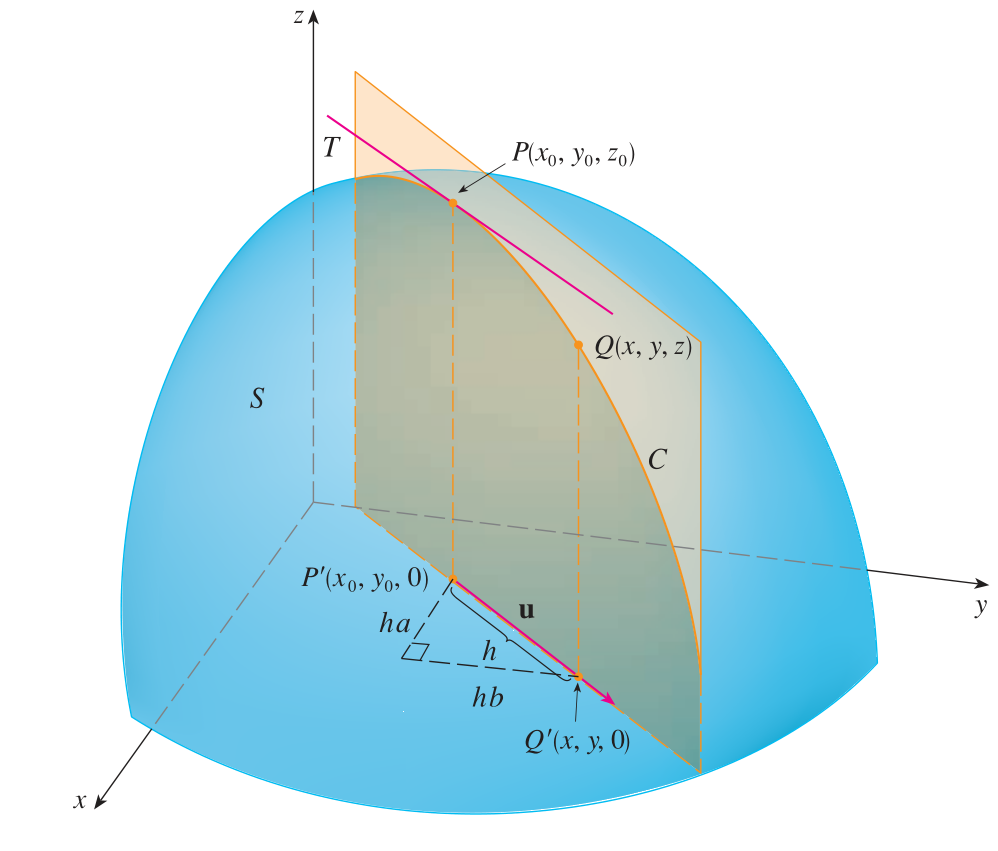
\includegraphics[width = 8 cm]{./images/grad.png}
  
\end{minipage}
\begin{minipage}[]{0.47\linewidth}
\subsection*{{\fontfamily{lmss}\selectfont \textcolor{blue5}{\faIcon{anchor} \underline{Directional Derivatives}}}}
We want the rate of change of $z$ at $(x _ 0, y _ 0 )$ in the direction of an unit vector \textbf{u} = $\langle a, b  \rangle$. 

\textcolor{blue5}{\faIcon{caret-right}} Consider the surface $S$ of $z = f(x,y)$, the vertical plane that passes through $P(x_0, y_0, z_0)$  in the direction of \textbf{u} intersects $S$ a curve $C$. 

\textcolor{blue5}{\faIcon{caret-right}} The slope of tangent line $T$ to $C$ at $P$ is what we need.
\end{minipage}

If $Q(x,y,z)$ is another point on $C$ and $P', Q'$ are the projections of $P, Q$ onto the $xy$-plane, then the vector $\vv{P'Q'}$ is parallel to \textbf{u}, 
\[\vv{P'Q'} = h \textbf{u} = \langle ha, hb  \rangle  \]
Therefore $x - x_0 = ha$, $y - y_0 = hb $.
\[ \cfrac{\Delta z }{h } = \cfrac{z - z_0 }{h } = \cfrac{f(x_0 + ha, y_0 + hb ) - f(x_0, y_0)}{h}\]
If we take limit as $h \to 0 $, we obtain the rate of change of $z $ (with respect to distance) in the direction of \textbf{u}.
\begin{Def}[Directional Derivatives]
  The \textbf{directional derivative} of $f $ at $(x_0, y_0 )$ in the direction of a unit vector \textbf{u} = $\langle a, b  \rangle$ is 
  \begin{align*}
    D_u f(x_0, y_0 ) & = \lim_{h \to 0 }\cfrac{f(x_0 + ha, y_0 + hb ) - f(x_0, y_0)}{h} \\
                     & = f_x(x,y) a + f_y (x,y) b \\
                     & = f_x(x,y) \cos{\theta} + f_y(x,y) \sin{\theta}  \quad \text{(\textbf{u} makes an angle $\theta$ with the $x^{+}$-axis)} 
  \end{align*}    
\end{Def}

\begin{minipage}[]{0.3\linewidth}
  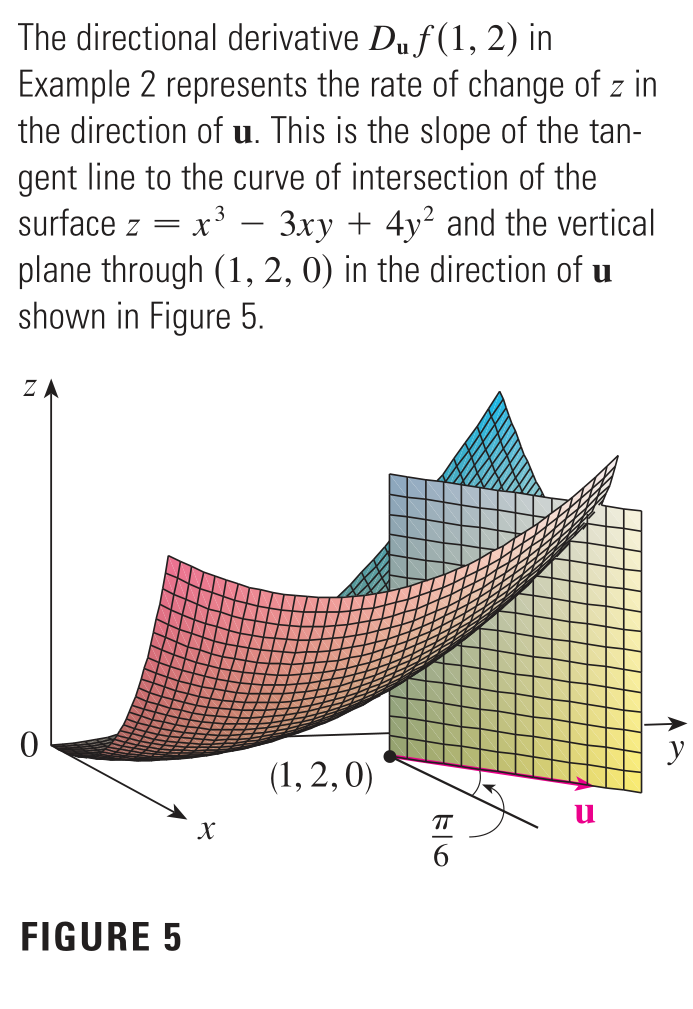
\includegraphics[width = 4.7 cm]{./images/grad2.png}
  
\end{minipage}
\begin{minipage}[]{0.67\linewidth}
{\fontfamily{lmtt}\selectfont \textbf{\textcolor{blue5}{\faIcon{map-marker-alt} EXAMPLE.}}} Find the directional derivative $D_uf(x,y)$ if \[f(x,y) = x^3 - 3xy + 4 y^2 \]
and \textbf{u} is given by $\theta = \pi/6$. What is $D_ \textbf{u} f(1,2)$?
 
{\fontfamily{lmtt}\selectfont \textbf{\textcolor{blue5}{SOLUTION.}}}  
$  f_x(x,y) = 3 x^2 - 3y \quad \text{ } \quad  f_y(x,y) = 8y -3 $

Therefore, 
\begin{equation*}
  \begin{split}
D_u f(x,y)  & = \cfrac{\sqrt{3 }}{2}(3 x^2 - 3y) + \cfrac{1 }{2 } (8y - 3)  \\
& = \cfrac{3 \sqrt{3 }}{2 } x^2 + \cfrac{4 - 3 \sqrt{3 }}{2 } y - \cfrac{3 }{ 2 }
  \end{split}
\end{equation*}
Hence $D_u f(1,2) = \cfrac{13 - 3 \sqrt{3 }}{2 }$
\end{minipage}
\pagebreak
\subsection*{{\fontfamily{lmss}\selectfont \textcolor{blue5}{\faIcon{anchor} \underline{The Gradient Vector}}}}
Notice that $D_ \textbf{u} = \langle f_x(x,y) , f_y(x,y) \rangle \cdot \textbf{u}$.
\begin{Def}[Gradient]
  The \textbf{gradient} of $f(x,y)$ is the vector function $\nabla f$ defined by 
  \[\nabla f(x,y) = \langle f_x (x,y) , f_y(x,y) \rangle = \cfrac{\partial f }{ \partial x } \textbf{i} + \cfrac{\partial f }{\partial y } \textbf{j}\]
  The directional derivative of $f(x,y)$ is $\quad D_ \textbf{u} f(x,y) = \nabla f(x,y) \cdot \textbf{u}$
\end{Def}
{\fontfamily{lmtt}\selectfont \textbf{\textcolor{blue5}{\faIcon{map-marker-alt} EXAMPLE.}}} If $f(x,y) = \sin{x} + e^{xy}$, then 
\begin{align*}
  & \nabla f(x,y) = \langle f_x, f_y  \rangle = \langle \cos{x} + y e^{xy}, xe^{xy} \rangle \\
  & \nabla f(0,1) = \langle 2, 0  \rangle
\end{align*}

\begin{minipage}[]{0.3\linewidth}
  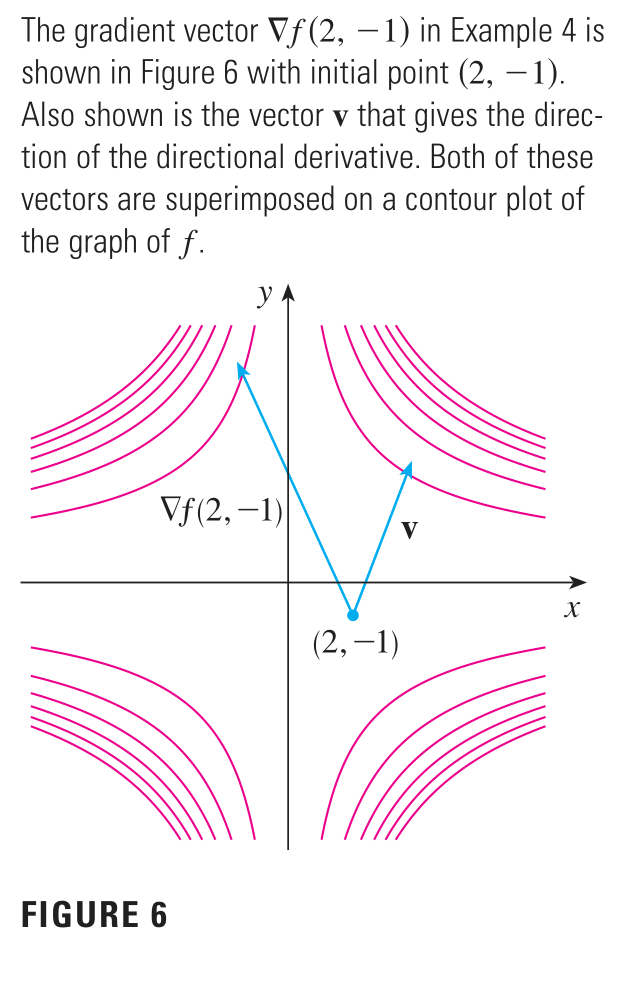
\includegraphics[width = 4.3 cm]{./images/grad4.png}
  
\end{minipage}
\begin{minipage}[]{0.67\linewidth}
  {\fontfamily{lmtt}\selectfont \textbf{\textcolor{blue5}{\faIcon{map-marker-alt} EXAMPLE.}}} Find the directional derivative of $f(x,y) = x^2 y^3 - 4y$ at $(2, -1 )$ in the direction of $\textbf{v} = 2 \textbf{i} + 5 \textbf{j}$.

  {\fontfamily{lmtt}\selectfont \textbf{\textcolor{blue5}{SOLUTION.}}} We first compute the gradient vector at $(2,-1)$: 
  \begin{align*}
    \nabla f(x,y) & = 2xy^3 \textbf{i} + (3 x^2 y^2 - 4 ) \textbf{i} \\
    \nabla f(2, -1) & = -4 \textbf{i} + 8 \textbf{j}
  \end{align*}
  The unit vector in the direction of \textbf{v} is $\textbf{u} = \cfrac{\textbf{v}}{|\textbf{v}|} = \cfrac{2 }{\sqrt{29 }} \textbf{ i} + \cfrac{5 }{\sqrt{29 }} \textbf{ j}$

  Therefore we have 
  \begin{align*}
    D_ \textbf{u} f(2,-1) & = \nabla f(2,-1) \cdot \textbf{u} = (-4 \textbf{i} + 8 \textbf{j}) \cdot \left( \cfrac{2 }{\sqrt{29 }} \textbf{ i} + \cfrac{5 }{\sqrt{29 }} \textbf{ j}  \right)\\
    & = \cfrac{-4 \cdot 2 + 8 \cdot 5  }{\sqrt{29}} = \cfrac{32 }{\sqrt{29 }}
  \end{align*}
\end{minipage}

\subsection*{{\fontfamily{lmss}\selectfont \textcolor{blue5}{\faIcon{anchor} \underline{Functions of Three Variables}}}}
\begin{Def}[Directional Derivatives]
  The \textbf{directional derivative} of $f$ at $(x_0, y_0, z_0)$ in the direction of a unit vector \textbf{u} $= \langle a, b, c  \rangle$ is 
  \[D_ \textbf{u} f(x_0, y_0, z_0) = \lim_{h \to 0 } \cfrac{f(x_0 + ha, y_0 + hb, z_0 + hc ) - f(x_0, y_0, z_0)}{h}\]
  The \textbf{gradient vector} is 
  \[\nabla f = \langle f_x, f_y, f_z  \rangle = \cfrac{\partial f }{ \partial x } \textbf{ i} + \cfrac{\partial f }{\partial y } \textbf{ j} + \cfrac{\partial f }{\partial z } \textbf{ k}  \]
  And the directional derivative is $\quad D_ \textbf{u} f(x,y,z) = \nabla f(x,y,z) \cdot \textbf{u}$
\end{Def} 
{\fontfamily{lmtt}\selectfont \textbf{\textcolor{blue5}{\faIcon{map-marker-alt} EXAMPLE.}}} If $f(x,y,z) = x \sin{yz}$, (a) find $\nabla f$ and (b) find $D_ \textbf{u} f(1,3,0)$ in the direction of $\textbf{v} = \textbf{i} + 2 \textbf{j}  - \textbf{k}$.

{\fontfamily{lmtt}\selectfont \textbf{\textcolor{blue5}{SOLUTION.}}} 
\[\nabla f = \sin{yz} \cdot \textbf{i} + xz\cos{yz} \cdot \textbf{j} + xy\cos{xz} \cdot \textbf{k}\]
The unit vector in the direction of \textbf{v} is 
\[\textbf{u} = \cfrac{1 }{\sqrt{6 }} \textbf{i} + \cfrac{2 }{\sqrt{6 }} \textbf{j} - \cfrac{1 }{\sqrt{6 }} \textbf{k}\]
Therefore 
\begin{align*}
  D _ \textbf{u} & = \nabla f(1,3,0) \cdot \textbf{u} \\
  & = 3 \textbf{k} \cdot \cfrac{1 }{\sqrt{6 }} \textbf{i} + \cfrac{2 }{\sqrt{6 }} \textbf{j} - \cfrac{1 }{\sqrt{6 }} \textbf{k} \\
  & = - \sqrt{\cfrac{3 }{2 }}
\end{align*}

\end{document}
